\chapter{实验 1: 渐进分析和排序算法}
%\addcontentsline{toc}{chapter}{实验 1: 渐进分析和排序算法}
\section{Task 1}

\begin{itemize}
	\item[(1)] 使用 $\t O,\Omega$ 和 $\Theta$ 的定义, 证明下面每一个等式:
	\begin{itemize}
		\item[a)] $2\sqrt n + 6 = \t O(\sqrt n)$
		\begin{proof}
			取 $C=8$ 则, $2\sqrt n + 6 \leq 8\sqrt n$ 故 $2\sqrt n + 6 = \t O(\sqrt n)$
		\end{proof}
		\item[b)] $n^2=\Omega(n)$
		\begin{proof}
			取 $C=1$ 则, $n^2\geq n$ 故 $n^2=\Omega(n)$.
		\end{proof}
		\item[c)] $\log_2(n)=\Theta(\ln (n))$
		\begin{proof}
			取 $C=\log_2 e$ 则, $\frac 1 C \log_2 (n)=\ln (n)$
			故 $\log_2 (n)=\Theta(\ln (n))$.
		\end{proof}
		\item[d)] $4^n\neq \t O(2^n)$
		\begin{proof}
			$\forall C>0,\ \exists n=\lceil \log_2 C\rceil \ s.t. 4^n\geq 2^n$ 故 $4^n\neq \t O(2^n)$
		\end{proof}
	\end{itemize}
	\item[(2)] 使用数学归纳法证明 $T(n)=\t O(n^2)$. 其中
	
	$
	T(n)=\left\{
	\begin{aligned}
		T(n-1)+2n, & n>1 \\
		3, & n=1
	\end{aligned}
	\right.
	$
	\begin{proof}
		$n=1$ 时, 取 $C=3$ 则, $T(1)=\t O(1)$.
		
		设 $n=k$ 时成立, 即 $T(k)=\t O(k^2)$
		
		则存在 $C>0$ 使得 $T(k)\le Ck^2$
		
		当 $n=k+1$ 时.
		
		$T(k+1)=T(k)+2(k+1) \le Ck^2+2k+2 = (C-1)k^2+(k+1)^2 + 1 \le C(k+1)^2$ 当 $C=3$ 时.
		
		综上 $T(n)=\t O(n^2)$.
	\end{proof}
\end{itemize}

\section{Task 2}

\subsection{算法设计}

先将所有点按照 $x_i$ 为第一关键字, $y_i$ 为第二关键字排序, 并以点 $p_m(m=\lfloor\frac n 2\rfloor)$ 为分界点, 拆分点集 $A_1,A_2$:

$A_1=\{p_i|i=0\ldots m\} \qquad A_2=\{p_i|i=m+1\ldots n-1\}$

并递归下去, 求出两点集各自内部的最近点对, 设距离为 $h_1,h_2$, 取较小值设为 $h$.

我们将所有横坐标与 $x_m$ 的差小于 $h$ 的点放入集合 $B=\{p_i| |x_i-x_m|<h \}$ 而只有这些点内部的点距离可能更优. 

同样的, 如果想比 $h$ 更小, $B$ 中点的纵坐标之差也得小于 $h$.

我们设 $C(p)=\{p_i|p_j\in B,y_i-h<y_j\le y_i\}$.

接下来只需对每对 $p_i\in B,p_j\in C(p_i)$ 求距离并取最小值即可.

至此我们已经完成了这个问题, 但还有一些实现的细节需要完善, 比如如何快速计算 $C$ 数组. 这将在复杂度分析中给出具体方式及其正确性证明.

\subsection{复杂度分析}

我们先来考虑 $C$ 的计算方式, 最朴素的想法就是将 $B$ 中的点按 $y_i$ 排序, 就可以得到.

但是如果每次直接排序, 这部分的复杂度就变为 $\t O(n\log ^2 n)$. 超出了预期.

但仔细思考后, 在求 $B$ 的时候我们已经不需要 $x_i$ 的顺序了, 所以在递归过程中我们可以利用归并排序对 $y$ 进行排序, 由此我们就可以在 $\t O(n\log n)$ 的时间复杂度内求出 $C$.

除此之外, 在每次求完 $C$ 并更新答案时我们的复杂度为 $|C|$, 而粗略看去 $|C|$ 应该是 $\t O(n)$ 级别, 那么总复杂度将退化为 $\t O(n^2)$. 但经过仔细分析后实则不然, $C$ 的大小并没有那么大, 最大大小实际上只有 $7$. 我们进一步考虑 $C$ 的定义, 发现 $C(p_i)$ 内部的点应该落在 $(x_m-h,x_m+h) \times (y_i-h,y_i]$ 这个大小为 $2h\times h$ 的矩形内, 而当我们以中心线 $x_m$ 将其分成两个部分. 

下面只考虑左半部分, 由于左半边被之前分治的左半边包含, 所以该区域内任意两点的距离应该不小于 $h$, 而该部分的面积为 $h\times h$. 更进一步的, 我们将这个 $h\times h$ 的矩形分成四个 $\frac h 2 \times \frac h 2$ 的小矩形, 则每个小矩形内部最多只会存在一个点, 因为小矩形的对角线长度也仅有 $\frac {h} {\sqrt 2}<h$ 所以在整个 $2h\times h$ 中最多只会存在 $8$ 个点, 再除去 $p_i$ 本身, 就只会剩下 $7$ 个点.

通过上述分析, 我们分治之后合并的复杂度是 $\t O(n)$.

那么总复杂度就是 $T(n)=2T(\frac n 2)+\t O(n)=\t O(n\log n)$.

\subsection{代码实现}

代码如下, 已通过洛谷 P7883 平面最近点对(加强加强版)

\begin{lstlisting}
const int N=4e5+10;
const ll INF=9e18;
int n;
struct Point{
	int x,y;
}a[N],b[N];
bool cmp(Point a,Point b)
{
	return a.x<b.x;
}
bool cmp2(Point a,Point b)
{
	return a.y<b.y;
}
ll dist(Point a,Point b)
{
	return 1ll*(a.x-b.x)*(a.x-b.x)+1ll*(a.y-b.y)*(a.y-b.y);
}
ll solve(int l,int r)
{
	if(r-l<=10)
	{
		ll ans=INF;
		sort(a+l,a+r+1,cmp2);
		for(int i=l;i<=r;i++)
		for(int j=i+1;j<=r;j++)
		ans=min(ans,dist(a[i],a[j]));
		return ans;
	}
	int mid=(l+r)>>1;
	int px=a[mid].x;
	ll ans=INF;
	ans=min(solve(l,mid),solve(mid+1,r));
	int p1=l,p2=mid+1,p3=l;
	while(p1<=mid&&p2<=r)
	{
		if(a[p1].y<a[p2].y)b[p3++]=a[p1++];
		else b[p3++]=a[p2++];
	}
	while(p1<=mid)b[p3++]=a[p1++];
	while(p2<=r)b[p3++]=a[p2++];
	for(int i=l;i<=r;i++)a[i]=b[i];
	int tot=0;
	for(int i=l;i<=r;i++)
	if(1ll*abs(a[i].x-px)*abs(a[i].x-px)<ans)
	{
		for(int j=tot;j&&1ll*(a[i].y-b[j].y)*(a[i].y-b[j].y)<ans;--j)
		ans=min(ans,dist(a[i],b[j]));
		b[++tot]=a[i];
	}
	return ans;
}
int main()
{
	read(n);
	for(int i=1;i<=n;i++)
	read(a[i].x),read(a[i].y);
	sort(a+1,a+n+1,cmp);
	cout<<solve(1,n);
	return 0;
}
\end{lstlisting}

\section{Task 3}

以下为各排序算法的主干代码. 均用 $50$ 组不同规模随机数据, 正序数据和逆序数据进行测试.

\subsection{插入排序}

\begin{lstlisting}
void Insertion(vector<int>&num)
{
	int n=num.size();
	for(int i=1;i<n;i++)
	{
		int pos=i;
		for(int j=i-1;j>=0;j--)
		if(num[i]<num[j])
			pos=j;
		int val=num[i];
		for(int j=i;j>pos;j--)num[j]=num[j-1];
		num[pos]=val;
	}
	return;
}
\end{lstlisting}

\subsection{选择排序}

\begin{lstlisting}
void Selection(vector<int>&num)
{
	int n=num.size();
	for(int i=0;i<n-1;i++)
	{
		int pos=i;
		for(int j=i;j<n;j++)
		if(num[j]<num[pos])pos=j;
		swap(num[i],num[pos]);
	}
	return;
}
\end{lstlisting}

\subsection{希尔排序}

\begin{lstlisting}
void Shell_1(vector<int>&num)
{
	static int H[30];
	int n=num.size(),p=0;
	H[p]=1;
	for(;H[p]<n;p++)
	H[p+1]=H[p]<<1;
	while (p>=0)
	{
		int h=H[p];
		for (int i = h; i < n; i++)
		for (int j = i; j >= h && num[j] < num[j - h]; j -= h)
		swap(num[j], num[j - h]);
		p--;
	}
	return;
}
\end{lstlisting}

其余两个希尔排序只有 $H$ 数组发生变化, 变化如下:

\begin{lstlisting}
for(;H[p]<n;p++)
	H[p+1]=((H[p]+1)<<1)-1;
\end{lstlisting}

\begin{lstlisting}
for(;H[p]<n;p++)
	H[p+1]=((H[p]<<1|1)*3-1)/2;
\end{lstlisting}

\subsection{快速排序}

\begin{lstlisting}
int depth=0;
void Quicksort(vector<int>&num,int l,int r,int dep)
{
	depth=max(depth,dep);
	if(l==r)return;
	int pos=random(l,r); //在 [l,r] 中随机选取点, 利用 c++ rand() 函数实现
	int p=num[pos];
	swap(num[pos],num[r]);
	int i=l,j=r-1;
	while(i<j)
	{
		while(i<j&&num[i]<p)i++;
		while(i<j&&num[j]>=p)j--;
		swap(num[i],num[j]);
	}
	if(num[i]>=num[r])swap(num[i],num[r]);
	else i++;
	if(l<i)Quicksort(num,l,i-1,dep+1);
	if(i+1<=r)Quicksort(num,i+1,r,dep+1);
	return;
}
\end{lstlisting}

\subsection{归并排序}

\begin{lstlisting}
void Mergesort(vector<int>&num,int l,int r)
{
	static vector<int>tmp;
	if(l==r)return;
	int mid=(l+r)>>1;
	Mergesort(num,l,mid);
	Mergesort(num,mid+1,r);
	if(tmp.size()<r-l+1)tmp.resize(r-l+1);
	int p1=l,p2=mid+1,p=0;
	while(p1<=mid&&p2<=r)
	{
		if(num[p1]<num[p2])tmp[p++]=num[p1++];
		else tmp[p++]=num[p2++];
	}
	while(p1<=mid)tmp[p++]=num[p1++];
	while(p2<=r)tmp[p++]=num[p2++];
	for(int i=l;i<=r;i++)num[i]=tmp[i-l];
}
\end{lstlisting}

\section{Task 4}

以下为各排序算法实际运行时间测试, 同一组数据采取运行 $20$ 次所需时间的平均值.

考虑到选择和插入排序的效率过慢, 故对其余算法进行了更大数据集的测试和单独的图表绘制. 以此更清晰的表示其余算法的效率差异.

\subsection{随机数据}

\begin{figure}[H]    % 常规操作\begin{figure}开头说明插入图片
	% 后面跟着的[htbp]是图片在文档中放置的位置,也称为浮动体的位置,关于这个我们后面的文章会聊聊,现在不管,照写就是了
	\centering            % 前面说过,图片放置在中间
	\subfloat[所有算法]   % 第一张子图的下标(注意:注释要写在[]中括号内)
	{
		\label{fig:subfig1}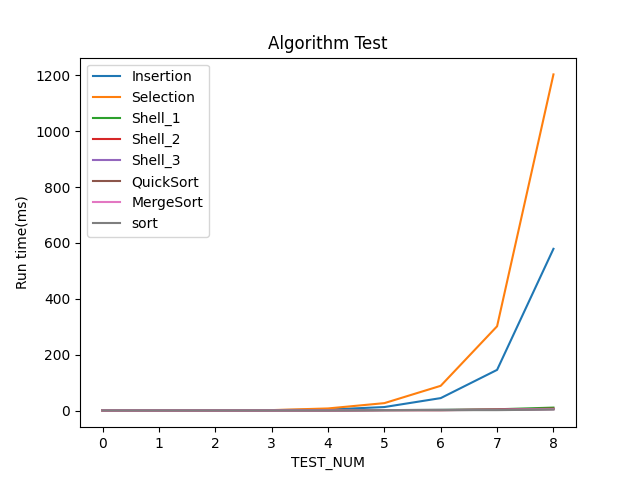
\includegraphics[width=0.4\textwidth]{figures/1_1.png}
	}
	\subfloat[去除插入和选择]
	{
		\label{fig:subfig2}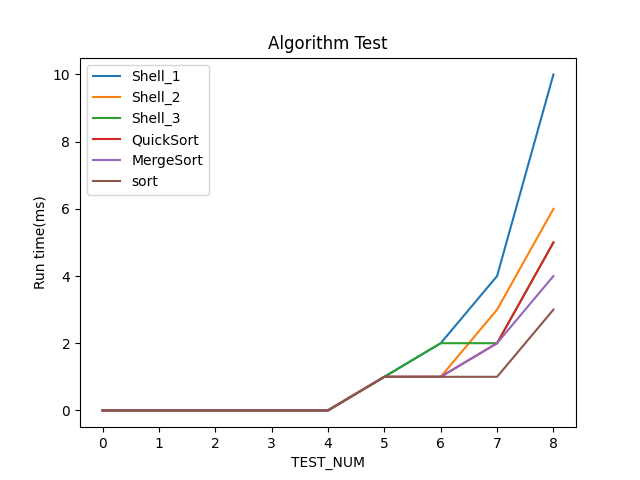
\includegraphics[width=0.4\textwidth]{figures/1_2.png}
	}
	\\
	\subfloat[更大测试数据]   % 第一张子图的下标(注意:注释要写在[]中括号内)
	{
		\label{fig:subfig3}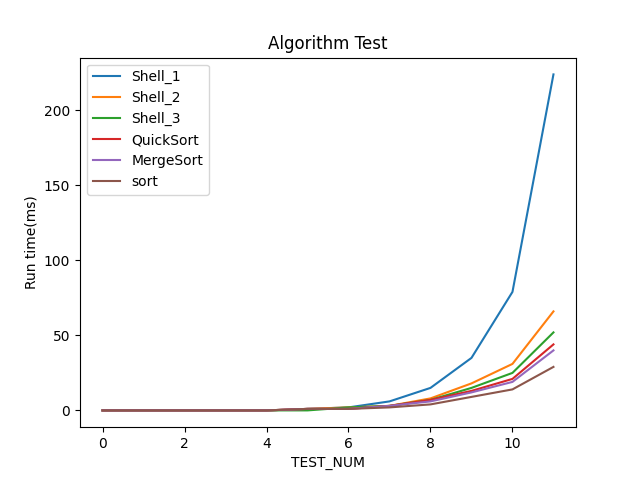
\includegraphics[width=0.4\textwidth]{figures/1_3.png}
	}
	\subfloat[更大测试数据并去除 Shell\_1]
	{
		\label{fig:subfig4}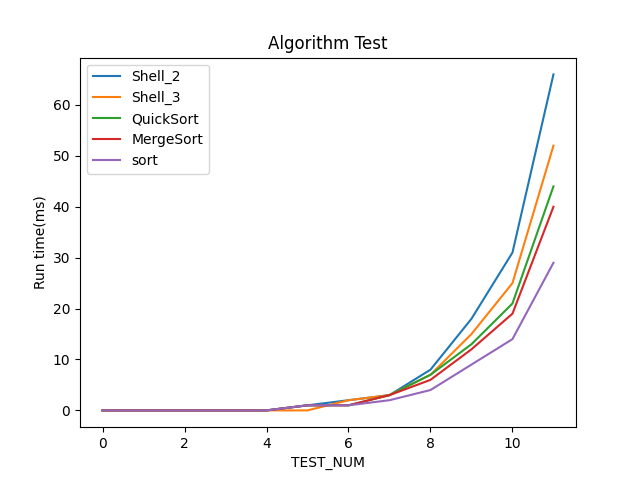
\includegraphics[width=0.4\textwidth]{figures/1_4.png}
	}
	\caption{随机数据}    % 整个图片的说明,注释写在{}内
	\label{fig:subfig_1}   
\end{figure}

\subsection{正序数据}

\begin{figure}[H]    % 常规操作\begin{figure}开头说明插入图片
		% 后面跟着的[htbp]是图片在文档中放置的位置,也称为浮动体的位置,关于这个我们后面的文章会聊聊,现在不管,照写就是了
		\centering            % 前面说过,图片放置在中间
		\subfloat[所有算法]   % 第一张子图的下标(注意:注释要写在[]中括号内)
		{
			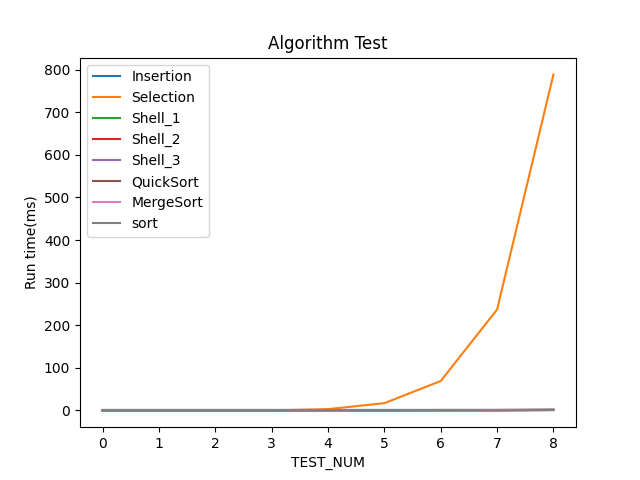
\includegraphics[width=0.4\textwidth]{figures/2_1.png}
		}
		\subfloat[去除插入和选择]
		{
			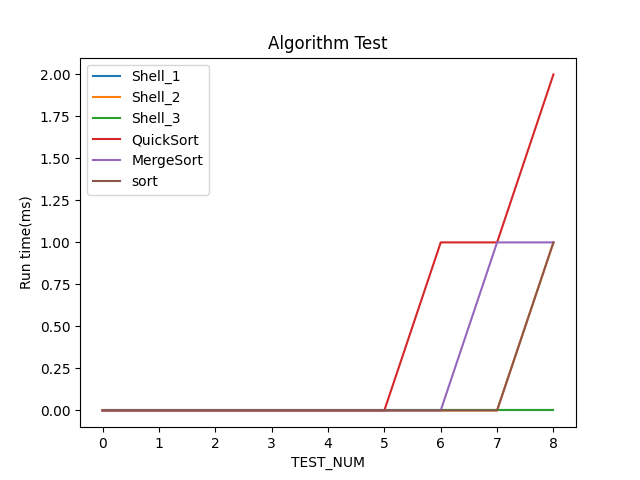
\includegraphics[width=0.4\textwidth]{figures/2_2.png}
		}
		\caption{正序数据}    % 整个图片的说明,注释写在{}内
		
\end{figure}

\subsection{逆序数据}

\begin{figure}[H]    % 常规操作\begin{figure}开头说明插入图片
		% 后面跟着的[htbp]是图片在文档中放置的位置,也称为浮动体的位置,关于这个我们后面的文章会聊聊,现在不管,照写就是了
		\centering            % 前面说过,图片放置在中间
		\subfloat[所有算法]   % 第一张子图的下标(注意:注释要写在[]中括号内)
		{
			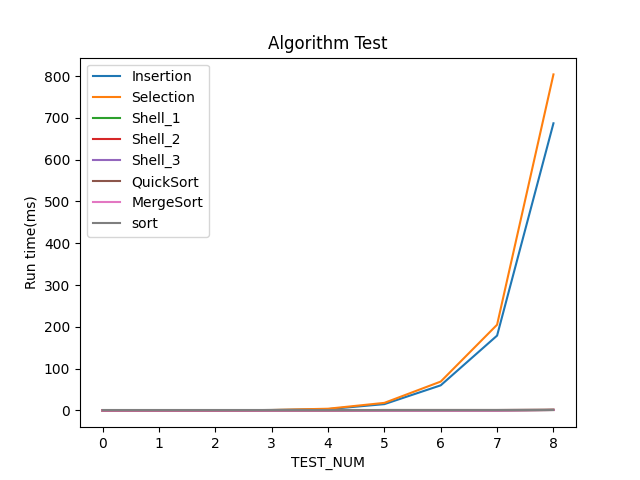
\includegraphics[width=0.4\textwidth]{figures/3_1.png}
		}
		\subfloat[去除插入和选择]
		{
			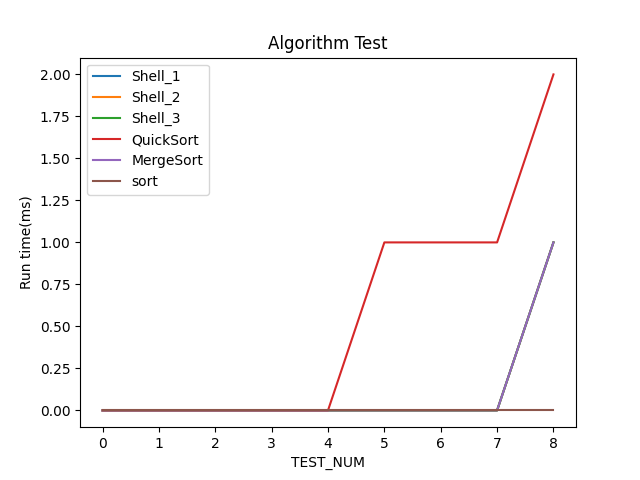
\includegraphics[width=0.4\textwidth]{figures/3_2.png}
		}
		\caption{逆序数据}    % 整个图片的说明,注释写在{}内
		
\end{figure}

\subsection{总结}

从理论分析上看, 插入排序和选择排序的时间复杂度均为 $\t O(n^2)$ 级别, 而快排和归并排序均为 $\t O(n\log n)$, 而实际测试中, 这两种算法的实际用时也确实远超过其余算法.

而对于希尔, 快排, 归并和 C++ stl 中的 sort 函数. Shell\_1 在小数据与其他算法时间差距不大, 但当数据规模进一步扩大后, 用时增长速度明显大于其余算法. 而 Shell\_2 在大数据规模下也有较差的表现.

而快排和归并, 则一直用时接近, 只有细微差别. C++ stl 中的 sort 函数表现出了较优的性能.

对于不同的数据性质选择, 快排, 归并和希尔用时变化不大. 

而插入排序, 如果是从后往前寻找插入位置时, 当数据为正序理论复杂度为 $\t O(n)$, 实际运行效率也很高.

\section{Task 5}

\subsection{快排层数}

\begin{figure}[H]
	\centering
	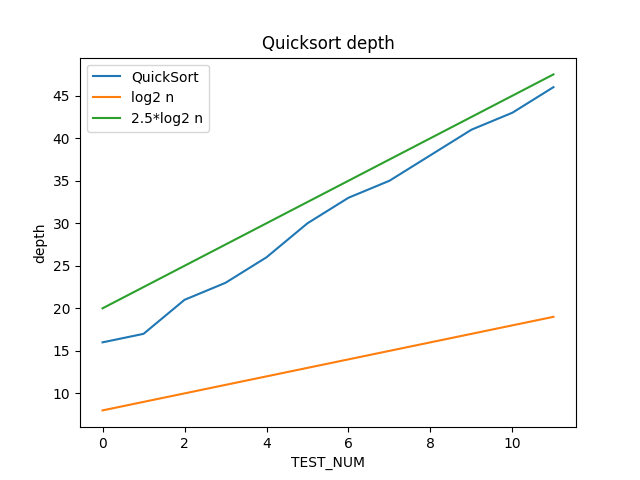
\includegraphics[width=0.8\textwidth]{figures/quick_dep.png}
\end{figure}

在 $2^8\sim 2^{19}$ 这 12 组数据测试结果中, 从图中可以看出递归深度大概是一个 $\t O(\log_2 n)$ 级别.

而从理论分析上看, 快排轴值的选取期望就是中间值, 故理论上递归层数就应该是 $\t O(\log_2 n)$ 级别.

\subsection{快排优化}

\begin{figure}[H]
	\centering
	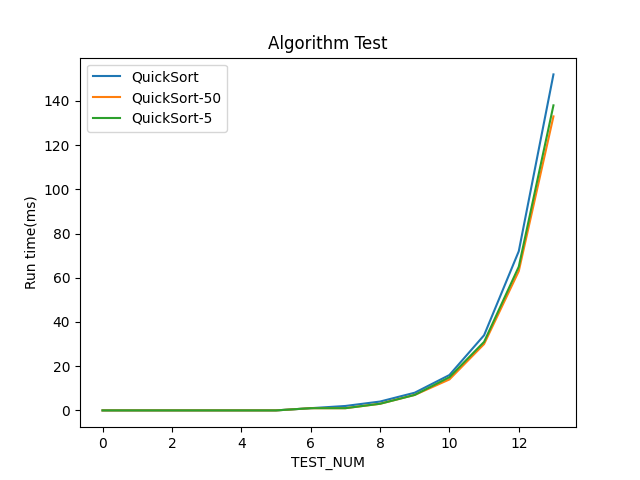
\includegraphics[width=0.8\textwidth]{figures/quick.png}
\end{figure}

通过设定阈值分别为 $50$ 和 $5$, 在 $2^8\sim 2^{21}$ 这些数据中, 可以看出, 优化过的两份算法均略优于没优化过的快排.
但优化幅度并不大, 只是常数上的优化, 并不影响算法复杂度.

而对于不同的阈值, 由此实验看出 $50$ 比 $5$ 快了几毫秒, 基本区别不大.

\subsection{螺丝螺母匹配问题}:
 
由于我们无法直接比较螺丝或螺母的大小, 所以考虑先找到一个轴值, 并利用轴值与相对的类别进行比较.

具体的, 类似快排, 我们先选取一个轴值螺母, 将这个螺母与区间内每个螺丝比较, 找到与该轴值螺母匹配的螺丝, 记为轴值螺丝.

接下来利用轴值螺母对所有螺丝做快排的操作, 利用轴值螺丝对所有螺母做快排的操作.

之后只需类似快排的递归调用即可.

程序实现:

 \begin{lstlisting}
 int match(int nut,int bolt)
 {
 	return nut==bolt?0:nut>bolt?1:-1;
 }
 void Quicksort(vector<int>&nuts,vector<int>&bolts,int l,int r)
 {
 	if(l==r)return;
 	int pos_nut=random(l,r);
 	int p_nut=nuts[pos];
 	int pos_bolt=l,p_bolt;
 	for(int i=l;i<=r;i++)
 	if(match(p_nut,bolts[i])==0)pos_bolt=i;
 	p_bolt=bolts[pos_bolt];
 	swap(nut[pos_nut],nut[r]);
 	swap(bolt[pos_bolt],bolt[r]);
 	int i=l,j=r-1;
 	while(i<j)
 	{
 		while(i<j&&match(nut[i],p_bolt)==-1)i++;
 		while(i<j&&match(nut[j],p_blot)>=0)j--;
 		swap(num[i],num[j]);
 	}
 	if(match(nut[i],p_bolt)==1)swap(nut[i],nut[r]);
 	else i++;
 	
 	i=l,j=r-1;
 	while(i<j)
 	{
 		while(i<j&&match(p_nut,bolt[i])==1)i++;
 		while(i<j&&match(p_nut,bolt[i])<=0)j--;
 		swap(num[i],num[j]);
 	}
 	
 	if(match(p_nut,bolts[i])==-1)swap(bolts[i],bolts[r]);
 	else i++;
 	if(l<i)Quicksort(nuts,bolts,l,i-1);
 	if(i+1<=r)Quicksort(nuts,bolts,i+1,r);
 	return;
 }
 \end{lstlisting}
